\documentclass{article}%
\usepackage[T1]{fontenc}%
\usepackage[utf8]{inputenc}%
\usepackage{lmodern}%
\usepackage{textcomp}%
\usepackage{lastpage}%
\usepackage[head=40pt,margin=0.5in,bottom=0.6in]{geometry}%
\usepackage{graphicx}%
%
\title{\textbf{Trabajadores de CVG Alcasa protestaron en Guayana~por tabulador salarial}}%
\author{El Nacional Web}%
\date{02/10/2018}%
%
\begin{document}%
\normalsize%
\maketitle%
\textbf{URL: }%
http://www.el{-}nacional.com/noticias/protestas/trabajadores{-}cvg{-}alcasa{-}inician{-}nueva{-}jornada{-}protesta{-}guayana\_253949\newline%
%
\textbf{Periodico: }%
EN, %
ID: %
253949, %
Seccion: %
Protestas\newline%
%
\textbf{Palabras Claves: }%
Protestas, Bolívar\newline%
%
\textbf{Derecho: }%
2.3%
, Otros Derechos: %
NO\_TIENE%
, Sub Derechos: %
2.3.4%
\newline%
%
\textbf{EP: }%
SI\newline%
\newline%
%
\textbf{\textit{Los manifestantes cerraron la entrada y salida cercanas al elevado de la empresa}}%
\newline%
\newline%
%
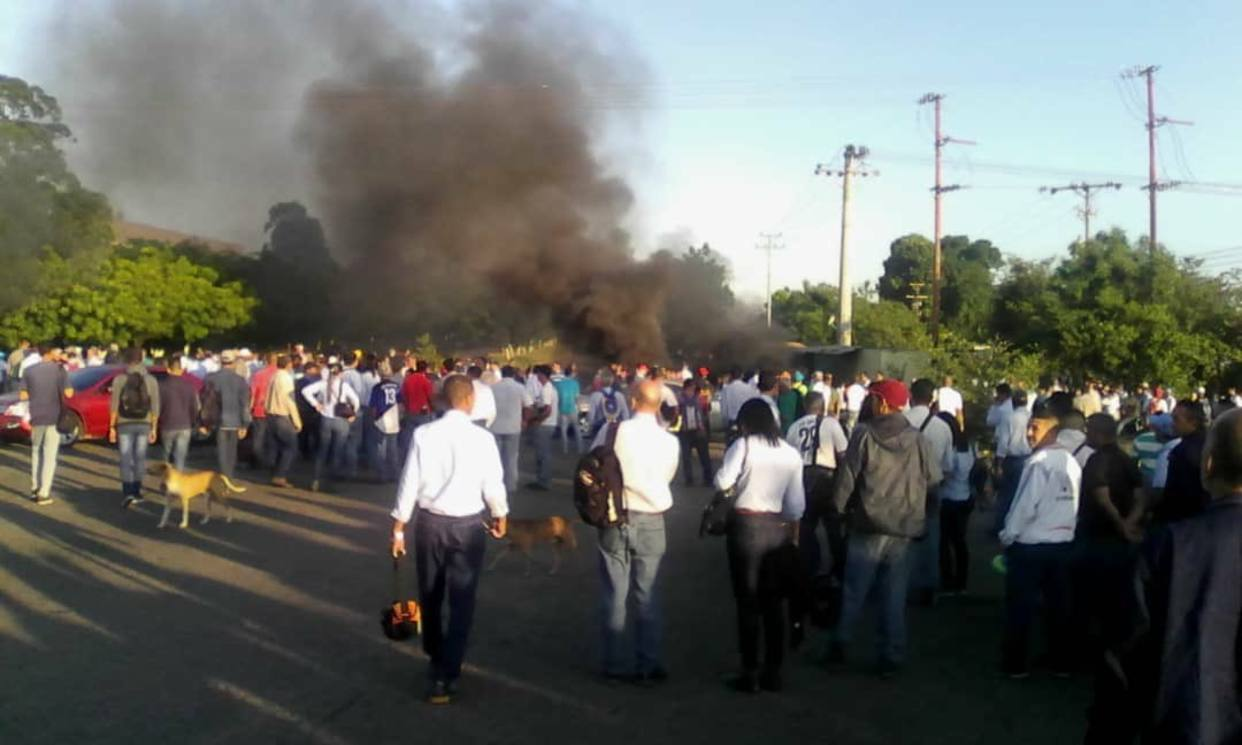
\includegraphics[width=300px]{245.jpg}%
\newline%
%
Trabajadores de las empresas básicas~de la industria CVG Alcasa iniciaron una nueva jornada de protestas este martes en Guayana, estado Bolívar.%
\newline%
%
Reportes de Twiter indican que desde las 6:00 am los manifestantes se concentraron en el lugar para exigir respeto por parte del gobierno al tabulador salarial.%
\newline%
%
Imágenes difundidas en Twitter muestran que los empleados quemaron cauchos y los colocaron en la vía para impedir en tránsito de vehículos.%
\newline%
%
Mantuvieron~cerrada la entrada y salida de la localidad, a la altura del elevado de Alcasa.%
\newline%
%
\end{document}